\documentclass[deutsch]{llncs}
\usepackage{multirow, cellspace}
\usepackage{microtype}
\usepackage{tabularx}
\usepackage{ltablex}
\usepackage{amssymb}
\usepackage{amsmath}
\usepackage[utf8]{inputenc} %Umlaute
\usepackage{amssymb}
\usepackage{upgreek}
\usepackage{graphicx}
\usepackage{amsmath}
\usepackage{array}

% subfigure
\usepackage{caption}
\usepackage{subcaption}
%


\renewcommand{\arraystretch}{1.5}
\renewcommand{\labelenumi}{\Alph{enumi}.}
\setlength{\jot}{10pt}

\begin{document}

\title{Intelligente Sehsysteme - Übungsblatt 2}


\author{Jan Konrad (2533619)}
\institute{}
\maketitle
\section{ImageToolBox: Gamma-Korrektur}
\begin{enumerate}
	\setcounter{enumi}{1}
	\item Eine Gamma-Korrektur mit $\gamma=3$ dunkelt das Bild ab. \\
	      Der Verlauf der Korrekturfunktion zeigt, dass niedrige Intensitätswerte gestaucht werden: $[0,0.5] \rightarrow [0,0.2]$\\
	      Hohe Intensitätswerte werden gespreizt: $[0.8,1] \rightarrow [0.5,1]$ \\

	      Eine Gamma-Korrektur mit $\gamma=1$ hat keinen Effekt. \\
	      Der Verlauf der Korrekturfunktion zeigt, dass jeder Intensitätswert unverändert bleibt: $T_\gamma(I)=I$ \\

	      Eine Gamma-Korrektur mit $\gamma=0.3$ hellt das Bild auf. \\
	      Der Verlauf der Korrekturfunktion zeigt, dass niedrige Intensitätswerte gespreizt werden: $[0,0.2] \rightarrow [0,0.6]$\\
	      Hohe Intensitätswerte werden gestaucht: $[0.5,1] \rightarrow [0.8,1]$
\end{enumerate}

\begin{figure}
	\centering
	\begin{subfigure}{.32\textwidth}
		\centering
		
\includegraphics[width=.99\linewidth]{A1/gamma=3.png}
		\caption{$\gamma=3$}
	\end{subfigure}
	\begin{subfigure}{.32\textwidth}
		\centering
		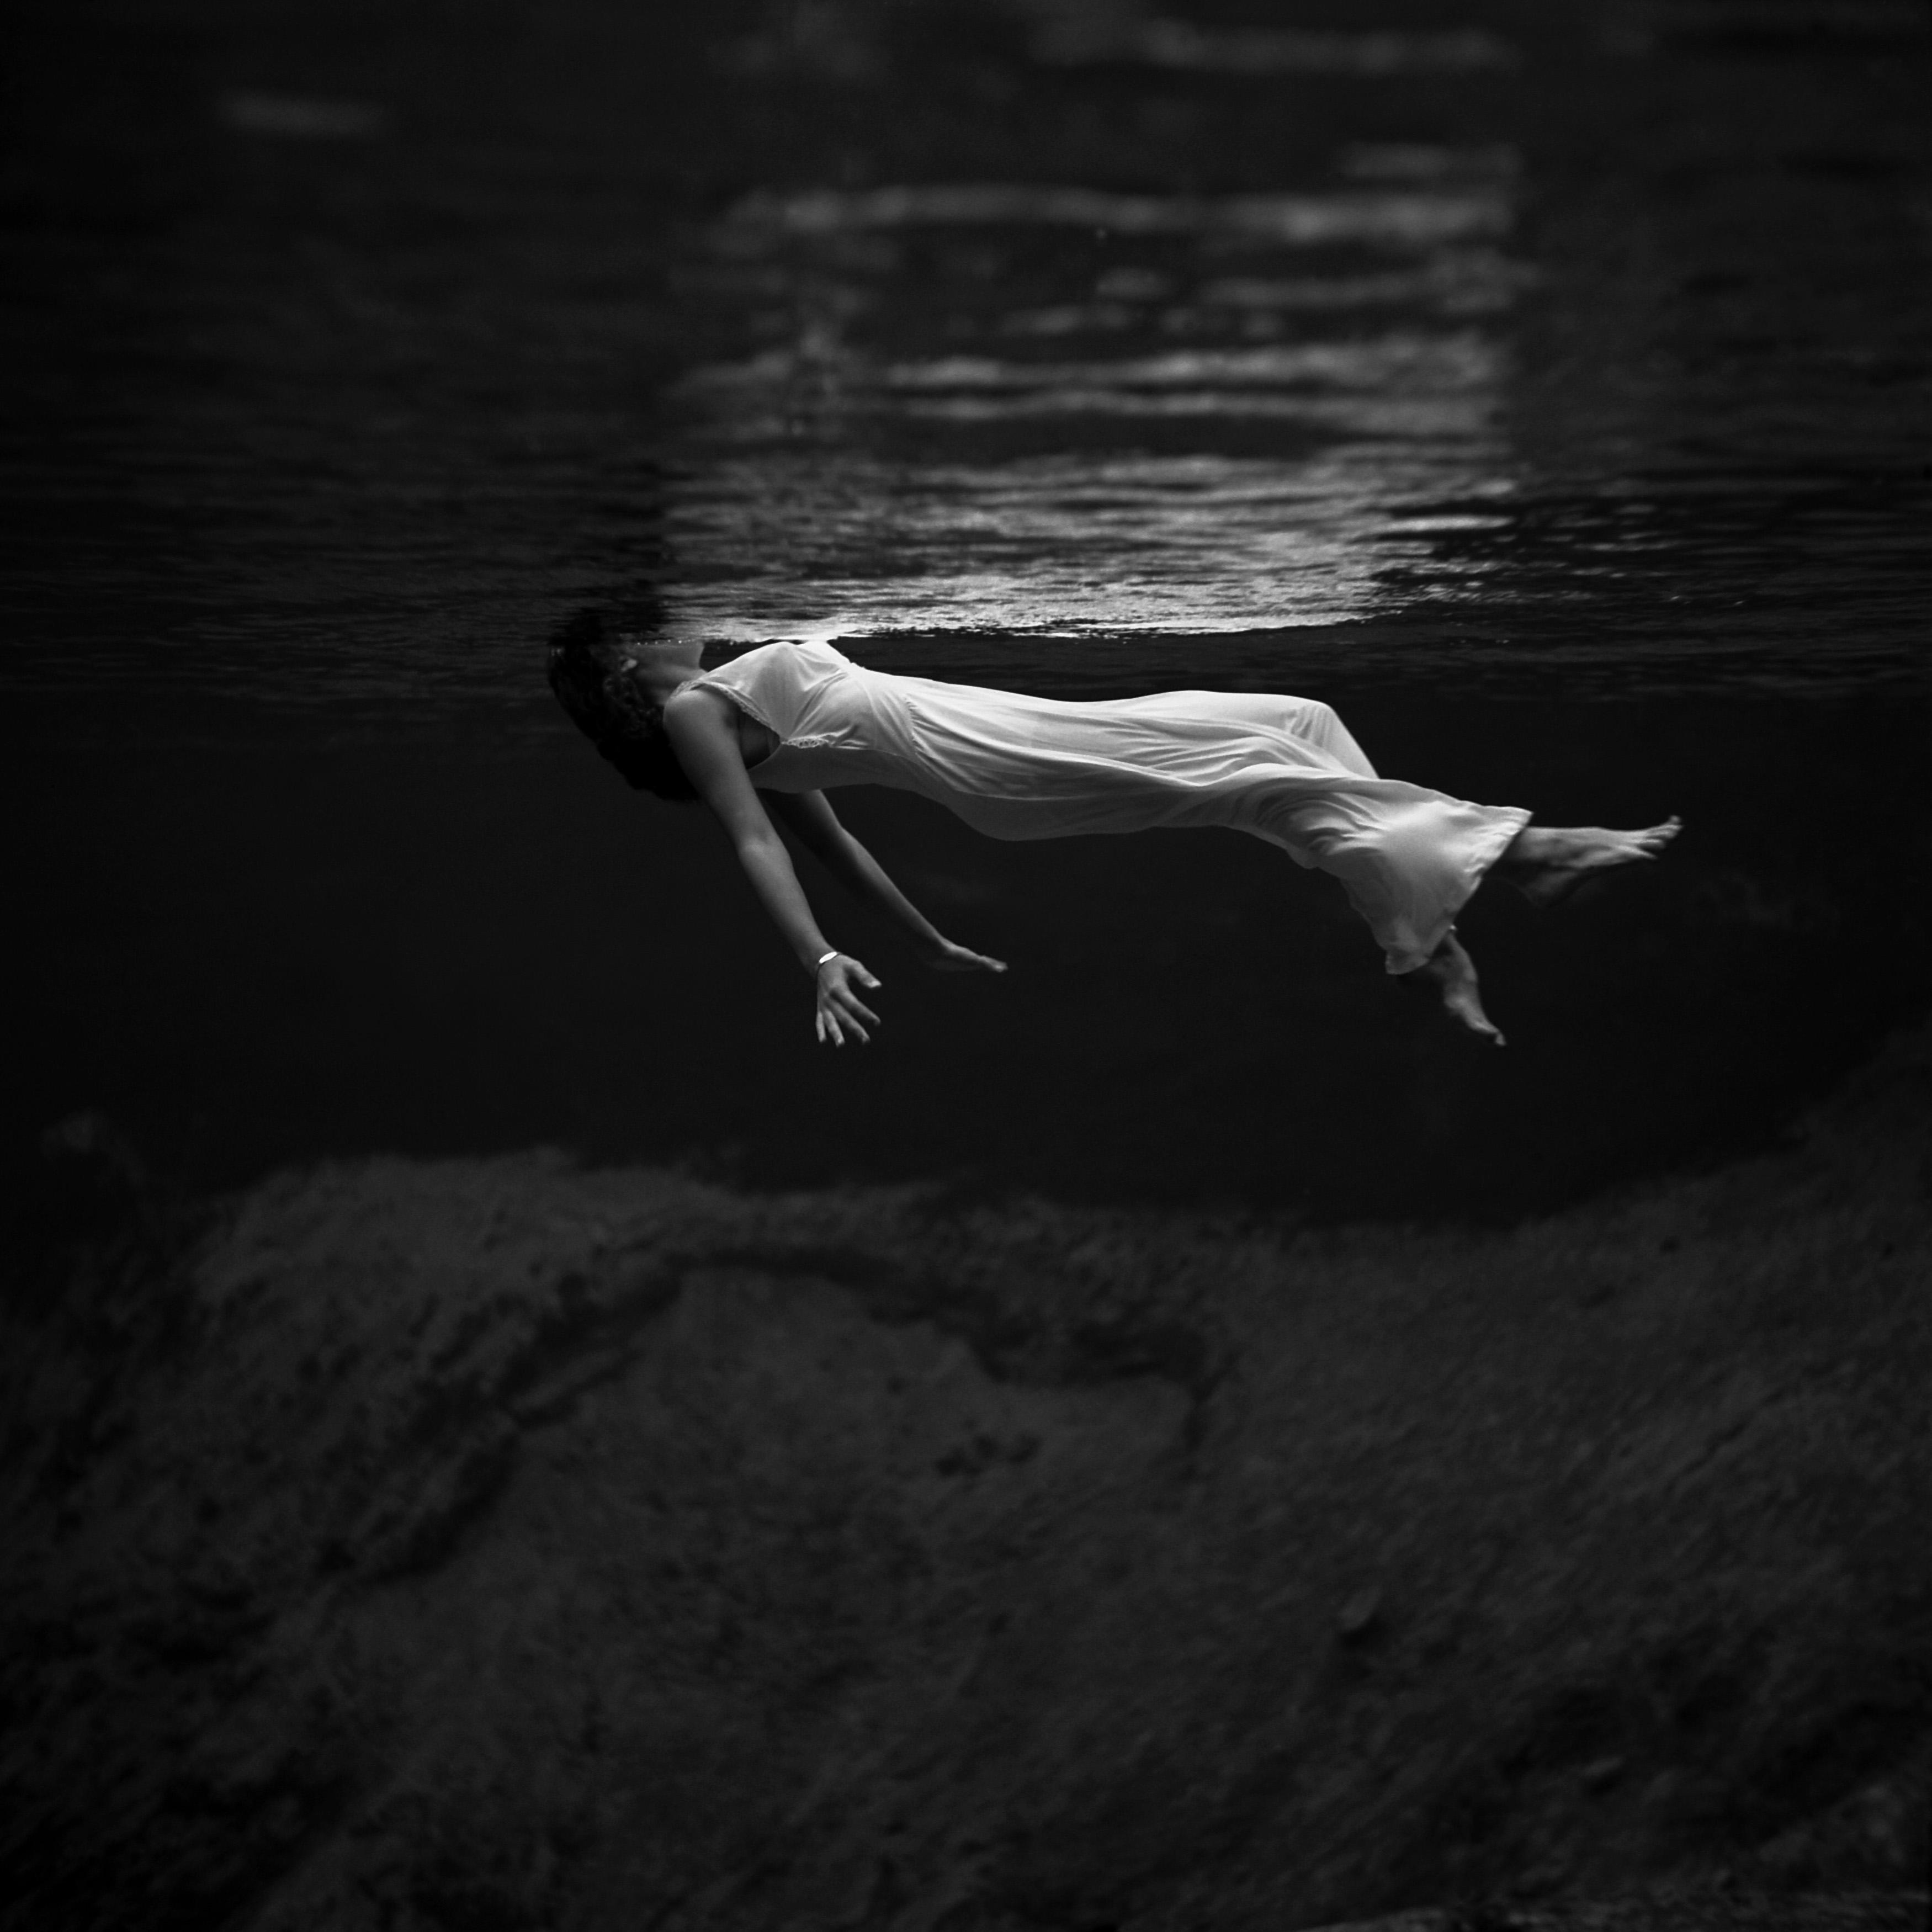
\includegraphics[width=.99\linewidth]{A1/gamma=1.png}
		\caption{$\gamma=1$}
	\end{subfigure}
	\begin{subfigure}{.32\textwidth}
		\centering
		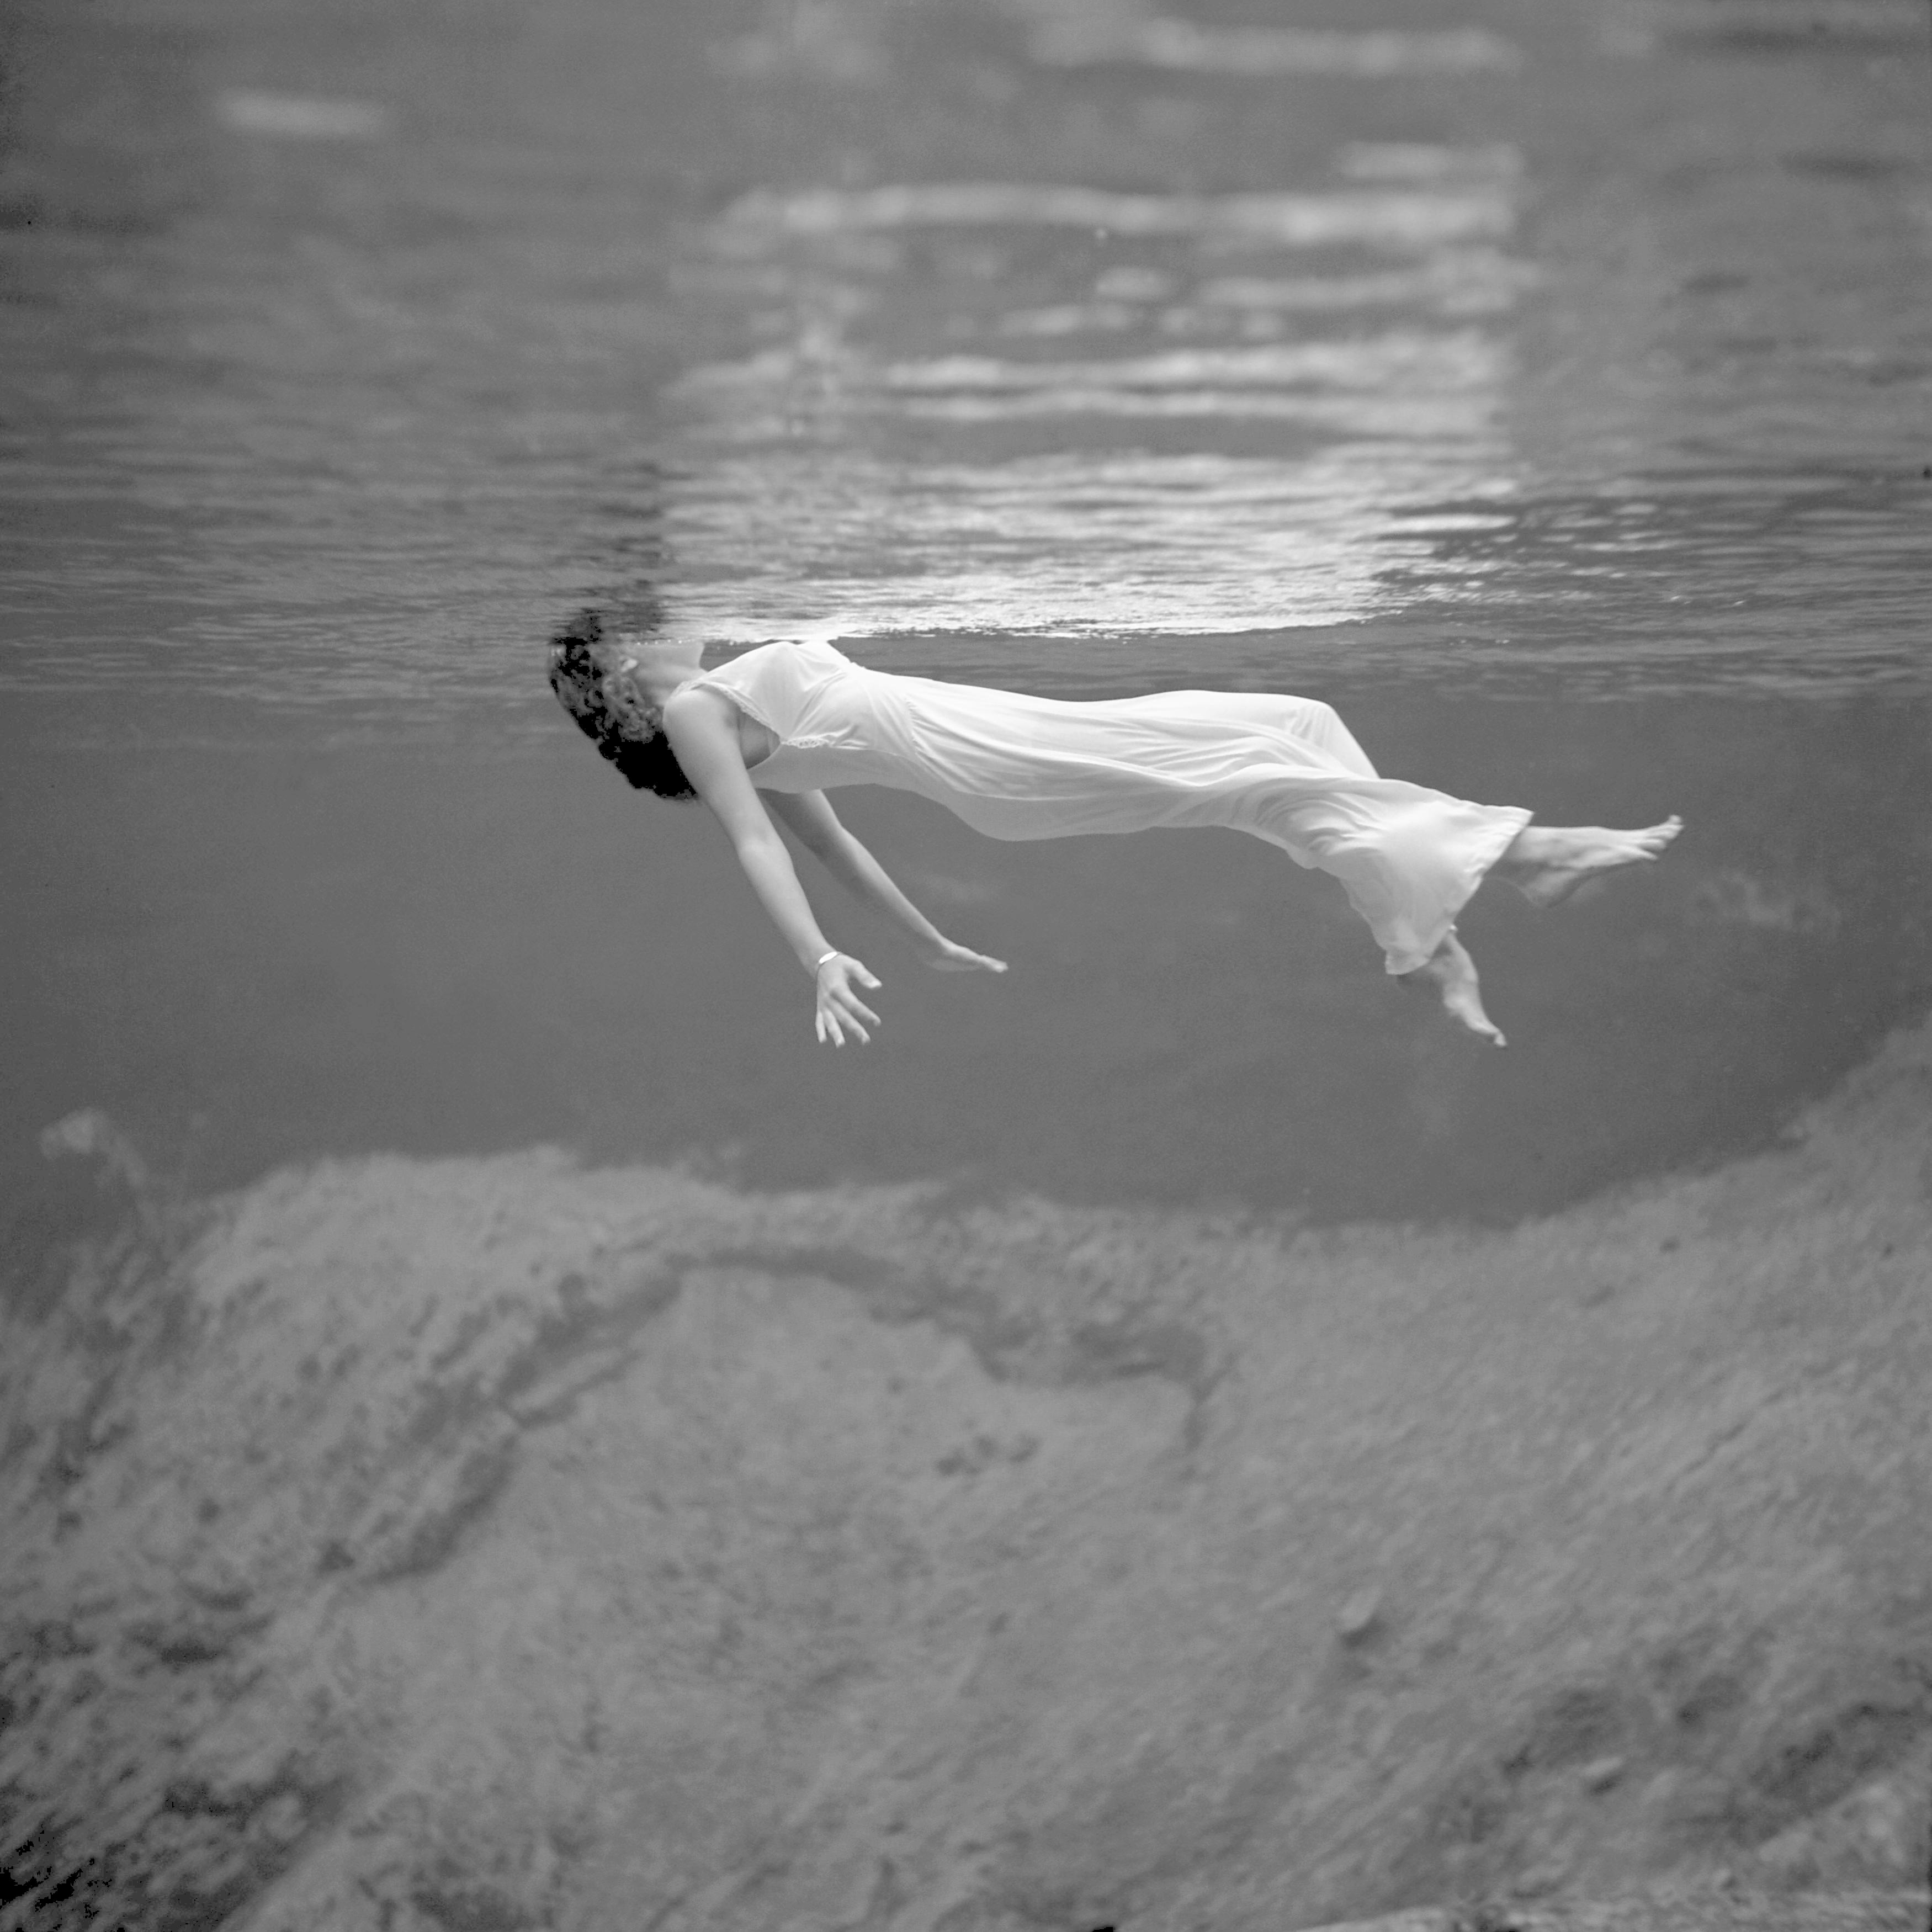
\includegraphics[width=.99\linewidth]{A1/gamma=0.3.png}
		\caption{$\gamma=0.3$}
	\end{subfigure}
\end{figure}

\newpage
\setcounter{section}{1}
\section{Korrespondierende Kosinus-Funktionen}
Für zwei an $N$ Orten abgetastete Funktionen $\cos(u_1\cdot n)$
und $\cos(u_2\cdot n)$ mit $ \frac{u_1}{u_0} = N - \frac{u_2}{u_0}$,
gilt: $\cos(u_1\cdot n)=\cos(u_2\cdot n)$ \\

\begin{equation}
	\label{cos1}
	\forall n \in \mathbb{Z}: \cos(x + 2\pi n) = \cos(x)
\end{equation}
\begin{equation}
	\label{cos2}
	\cos(-x ) = \cos(x)
\end{equation} \\
\begin{equation}
	\label{u1}
	\begin{alignedat}{3}
		& \frac{u_1}{u_0} & = & N - \frac{u_2}{u_0} \\
		\iff                                   & u_1             & = & N \cdot u_0 - u_2   \\
		\stackrel{u_0 = \frac{2 \pi}{N}}{\iff} & u_1             & = & 2\pi - u_2          \\
	\end{alignedat}
\end{equation} \\

\begin{equation}
	\begin{aligned}
		                                  & \cos(u_1\cdot n)            \\
		\stackrel{\text{(\ref{u1})}}{=}   & \cos(2\pi  n - u_2 \cdot n) \\
		\stackrel{\text{(\ref{cos1})}}{=} & \cos( - u_2 \cdot n)        \\
		\stackrel{\text{(\ref{cos2})}}{=} & \cos( u_2 \cdot n)          \\
	\end{aligned}
\end{equation}

\setcounter{section}{2}
\section{ImageToolBox: Diffusionsfilter }

\begin{figure}
	\centering
	\begin{subfigure}{.49\textwidth}
		\centering
		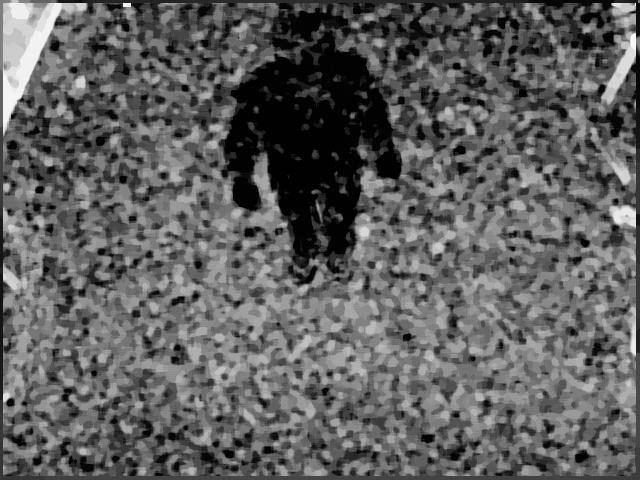
\includegraphics[width=.99\linewidth]{A3/lambda0.5.jpg}
		\caption{$\lambda=0.5$}
	\end{subfigure}
	\begin{subfigure}{.49\textwidth}
		\centering
		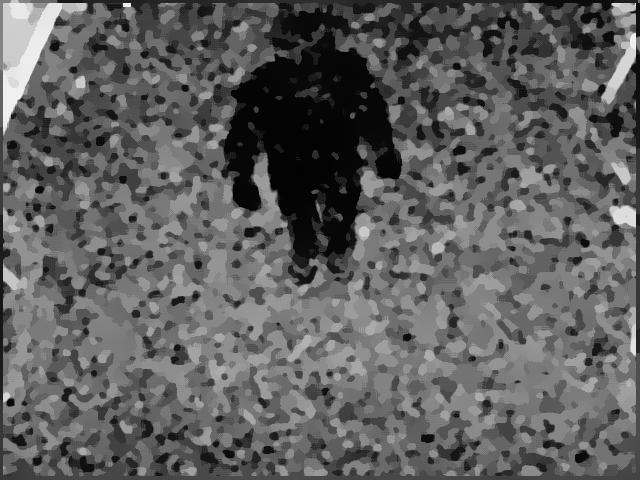
\includegraphics[width=.99\linewidth]{A3/lambda1.jpg}
		\caption{$\lambda=1$}
	\end{subfigure}
	\begin{subfigure}{.49\textwidth}
		\centering
		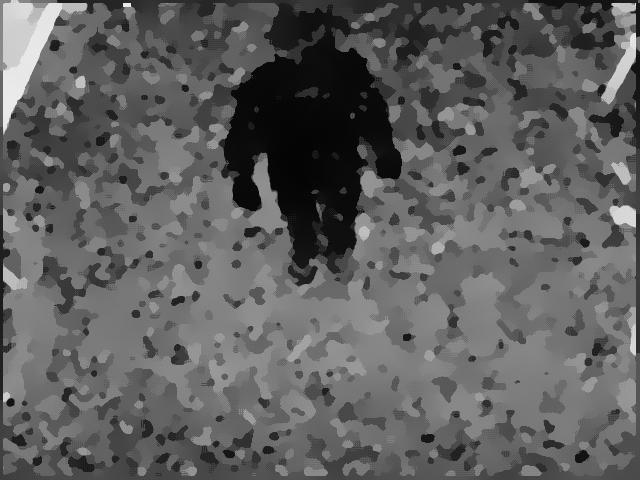
\includegraphics[width=.99\linewidth]{A3/lambda1.5.jpg}
		\caption{$\lambda=1.5$}
	\end{subfigure}
	\begin{subfigure}{.49\textwidth}
		\centering
		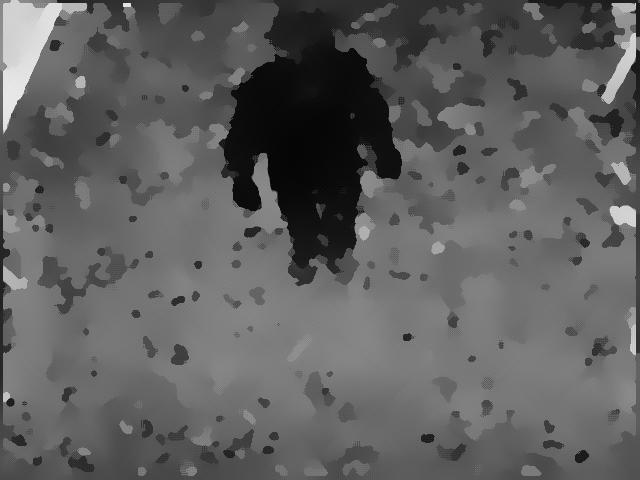
\includegraphics[width=.99\linewidth]{A3/lambda2.jpg}
		\caption{$\lambda=2$}
	\end{subfigure}

	\caption{Isotropes inhomogenes Diffusionsfilter mit $\epsilon_0=1$ und 500 Iterationen}
\end{figure}

\end{document}
